\whiteBGstarBegin
\setcounter{section}{0}
\section{Trắc nghiệm}
\begin{enumerate}[label=\bfseries Câu \arabic*:]
	
	\item \mkstar{1}
	
	\cauhoi
	{Đối với một vật quay quanh một trục cố định, câu nào sau đây là đúng?
		\begin{mcq}
			\item Nếu không chịu momen lực tác dụng thì vật phải đứng yên.
			\item Khi không còn momen lực tác dụng thì vật đang quay sẽ lập tức dừng lại.
			\item Vật quay được là nhờ có momen lực tác dụng lên nó.
			\item Khi thấy tốc độ góc của vật thay đổi thì chắc chắn đã có momen lực tác dụng lên vật.
		\end{mcq}
	}
	
	\loigiai
	{	\textbf{Đáp án: D.}
		
	Khi thấy tốc độ góc của vật thay đổi thì chắc chắn đã có momen lực tác dụng lên vật.	
	}
	\item \mkstar{1}
	
	\cauhoi
	{Chọn đáp án đúng. Mức quán tính của một vật quay quanh một trục \textbf{không} phụ thuộc vào
		\begin{mcq}(2)
			\item khối lượng của vật.
			\item hình dạng và kích thước của vật.
			\item tốc độ góc của vật.
			\item vị trí của trục quay.
		\end{mcq}
	}
	
	\loigiai
	{	\textbf{Đáp án: C.}
		
		Momen quán tính của vật phụ thuộc vào khối lượng của vật và sự phân bố khối lượng đó đối với trục quay, không phụ thuộc vào tốc độ góc của vật.
	}
	
	\item \mkstar{2}
	
	\cauhoi
	{Một vật đang quay quanh một trục với tốc độ góc $\omega =\SI{6.28}{\radian/\second}$. Nếu bỗng nhiên momen lực tác dụng lên nó mất đi thì 
		\begin{mcq}
			\item vật dừng lại ngay.
			\item vật đổi chiều quay.
			\item vật quay đều với tốc độ góc $\omega =\SI{ 6,28}{ \radian/\second}$.
			\item vật quay chậm dần rồi dừng lại.
		\end{mcq}
	}
	
	\loigiai
	{	\textbf{Đáp án: C.}
		
	Ta áp dụng lý thuyết mức quán tính trong chuyển động quay. 
	
	Một vật đang quay quanh một trục với tốc độ góc $\omega = \SI{6,28}{\radian/\second}$. Nếu bỗng nhiên momen lực tác dụng lên nó mất đi thì vật quay đều với tốc độ góc $\omega =\SI{ 6,28}{\radian/\second}$.
	}
	\item \mkstar{3}
	
	\cauhoi
	{Hùng và Dũng cùng nhau đẩy một chiếc thùng đựng hàng có trọng lượng $\SI{1200}{N}$ theo cùng chiều. Hùng đẩy với một lực $\SI{400}{N}$. Dũng đẩy với một lực $\SI{300}{N}$. Hệ số ma sát trượt giữa vật và sàn nhà là $\mu = \SI{0.2}{}$. Giá trị gần đúng nhất của gia tốc trong chuyển động tịnh tiến của thùng là (lấy $g=\SI{10}{m/s^2}$)
		\begin{mcq}(4)
			\item $\SI{0.38}{m/s^2}$.
			\item $\SI{0.038}{m/s^2}$.
			\item $\SI{3.8}{m/s^2}$.
			\item $\SI{4.6}{m/s^2}$.
		\end{mcq}
	}
	
	\loigiai
	{	\textbf{Đáp án: C.}
		
	Áp dụng định luật II Niu-tơn:
	$$\vec F_1 + \vec F_2 + \vec P + \vec N + \vec F_\text{ms} = m \vec a$$
	
	Trên phương $\text Oy$:
	$$N=P = \SI{1200}{N}$$
	
	Trên phương $\text Ox$:
	$$F_1 + F_2 - F_\text{ms} = ma \Rightarrow \Rightarrow F_1 + F_2 - \mu N = ma \Rightarrow a = \SI{3.83}{m/s^2}$$
	}
	\item \mkstar{4}
	
	\cauhoi
	{Một vật rắn có khối lượng $m=\SI{10}{kg}$ được kéo trượt tịnh tiến trên mặt sàn nằm ngang bởi lực $F$ có độ lớn $\SI{20}{N}$ hợp với phương nằm ngang một góc $\alpha = 30^\circ$. Cho biết hệ số ma sát trượt giữa vật và sàn là $\mu = \SI{0.1}{}$.Tính quãng đường vật đi được sau $\SI{4}{s}$ ($g=\SI{10}{m/s^2}$).
		\begin{mcq}(4)
			\item $\SI{6.21}{m}$.
			\item $\SI{6.42}{m}$.
			\item $\SI{6.65}{m}$.
			\item $\SI{6.72}{m}$.
		\end{mcq}
	}
	
	\loigiai
	{	\textbf{Đáp án: C.}
	
	\begin{center}
		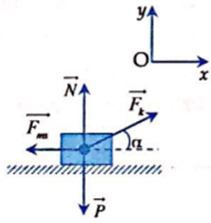
\includegraphics[scale=1]{../figs/VN10-2021-PH-TP024-4.png}
	\end{center}
	Chọn chiều dương trục $\text O x$ hướng theo phương chuyển động, trục $\text O y$ hướng theo phương trọng lực.
		
	Áp dụng định luật II Niu-tơn:
	$$\vec F + \vec P + \vec N + \vec F_\text{ms} = m \vec a$$
	
	Trên phương $\text Oy$:
	$$N = P - F \sin \alpha$$
	
	Trên phương $\text Ox$:
	$$F \cos \alpha - F_\text{ms} = ma \Rightarrow F \cos \alpha  - \mu (P-F \sin \alpha) = ma \Rightarrow a=\SI{0.83}{m/s^2}$$
	
	Vậy $s=\dfrac{1}{2}at^2 = \SI{6.65}{m}$.
	}
	
\end{enumerate}

\whiteBGstarEnd

\loigiai
{
	\begin{center}
		\textbf{BẢNG ĐÁP ÁN}
	\end{center}
	\begin{center}
		\begin{tabular}{|m{2.8em}|m{2.8em}|m{2.8em}|m{2.8em}|m{2.8em}|m{2.8em}|m{2.8em}|m{2.8em}|m{2.8em}|m{2.8em}|}
			\hline
			1.D  & 2.C  & 3.C  & 4.C  & 5.C  & & & & &  \\
			\hline
			
		\end{tabular}
	\end{center}
}
\section{Tự luận}
\begin{enumerate}[label=\bfseries Câu \arabic*:]
	\item \mkstar{1}
	
	\cauhoi{
	Momen lực có tác dụng như thế nào đối với một vật quay quanh một trục cố định? Mức quán tính của một vật quay quanh một trục phụ thuộc những yếu tố nào?
	}
	
	\loigiai{
		Momen lực tác dụng vào một vật quay quanh một trục cố định làm thay đổi tốc độ góc của vật.
		
		Mức quán tính của một vật quay quanh một trục phụ thuộc vào khối lượng của vật và sự phân bố khối lượng đó đối với trục quay.
	}
	
	\item \mkstar{2}
	
	\cauhoi
	{Có thể áp dụng định luật II Niu-tơn cho chuyển động tịnh tiến của một vật rắn được không? Tại sao?
	}
	
	\loigiai
	{
	Có thể áp dụng định luật II Niu-tơn cho chuyển động tịnh tiến của vật rắn. Vì tất cả các điểm của vật đều chuyển động với cùng một gia tốc, nên có thể xem vật rắn như một chất điểm.
	}
	\item \mkstar{3}
	
	\cauhoi
	{Một vật có khối lượng $m=\SI{40}{kg}$ bắt đầu trượt trên sàn nhà dưới tác dụng của một lực nằm ngang $F=\SI{200}{N}$. Hệ số ma sát trượt giữa vật và sàn là $\mu _\text t = \SI{0.25}{}$. Hãy tính:
		\begin{enumerate}
			\item Gia tốc của vật;
			\item Vận tốc của vật ở cuối giây thứ 3;
			\item Đoạn đường mà vật đi được trong 3 giây đầu.
		\end{enumerate}
	Lấy $g=\SI{10}{m/s^2}$.
	}
	
	\loigiai
	{		\begin{enumerate}
			\item Gia tốc của vật;
			
	Chọn hệ trục tọa độ $\text Oxy$ có O trùng với vị trí vật khi vật bắt đầu chuyển động. Chiều dương là chiều chuyển động.
	
	Áp dụng định luật II Niu-tơn:
	$$\vec P + \vec F + \vec N + \vec F_\text{ms} = m \vec a$$
	
	Chiếu lên $\text O x$:
	$$F-F_\text{ms} = ma$$
	
	Chiếu lên $\text O y$:
	$$N=P=mg$$
	
	Suy ra:
	$$F-\mu m g = ma \Rightarrow a = \SI{2.5}{m/s^2}$$
			\item Vận tốc của vật ở cuối giây thứ 3;
			
	$$v=at = \SI{7.5}{m/s}$$
	
			\item Đoạn đường mà vật đi được trong 3 giây đầu.
			
	$$s_3 = \dfrac{1}{2} at^2 = \SI{11.25}{m}$$
		\end{enumerate}
	}
	\item \mkstar{4}
	
	\cauhoi
	{Hai vật $m_1$ và $m_2$ được nối với nhau qua ròng rọc như hình vẽ.
		\begin{center}
			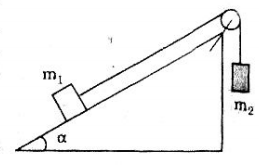
\includegraphics[scale=1]{../figs/VN10-2021-PH-TP024-1.png}
		\end{center}
	Hệ số ma sát giữa vật $m_1$ và mặt phẳng nghiêng là $\mu$. Bỏ qua khối lượng của ròng rọc và dây nối. Dây nối không giãn. Tính tỉ số $m_2 / m_1$ để vật $m_1$ đi lên thẳng đều.
	}
	
	\loigiai
	{		\begin{center}
			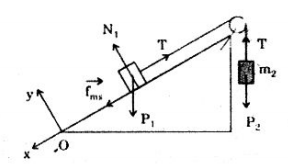
\includegraphics[scale=1.2]{../figs/VN10-2021-PH-TP024-2.png}
		\end{center}
		
		Vì vật chuyển động thẳng đều:
		$$\vec P_1 + \vec N_1 + T + \vec F_\text{ms} = 0$$
		
		Trên phương $\text Ox$:
		$$P_1 \sin \alpha - T + F_\text{ms} = 0 \Rightarrow P_2 \sin \alpha - P_2 + \mu N_1 = 0$$
		
		Trên phương $\text Oy$:
		$$N_1 = P_1 \cos \alpha$$
		
		Suy ra:
		$$P_1 \sin \alpha - P_2 + \mu P_1 \cos \alpha = 0 \Rightarrow P_1 (\sin \alpha + \mu \cos \alpha) = P_2 \Rightarrow \dfrac{P_2}{P_1} = \dfrac{m_2}{m_1} = \sin \alpha + \mu \cos \alpha$$
	}
	\item \mkstar{4}

\cauhoi
{Hai vật $m_1$ và $m_2$ được nối với nhau qua ròng rọc như hình vẽ.
	\begin{center}
		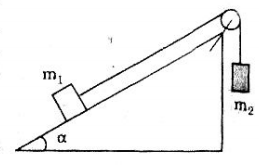
\includegraphics[scale=1]{../figs/VN10-2021-PH-TP024-1.png}
	\end{center}
	Hệ số ma sát giữa vật $m_1$ và mặt phẳng nghiêng là $\mu$. Bỏ qua khối lượng của ròng rọc và dây nối. Dây nối không giãn. Tính tỉ số $m_2 / m_1$ để vật $m_1$ đi xuống thẳng đều. Từ đố suy ra điều kiện $m_2 / m_1$ để vật $m_1$ đứng yên.
}

\loigiai
{		\begin{center}
		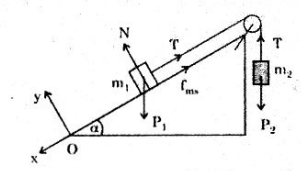
\includegraphics[scale=1.2]{../figs/VN10-2021-PH-TP024-3.png}
	\end{center}
	
	Lực ma sát hướng lên theo phương mặt phẳng nghiêng.
	
	Vì vật chuyển động thẳng đều:
	$$\vec P_1 + \vec N_1 + T + \vec F_\text{ms} = 0$$
	
	Trên phương $\text Ox$:
	$$P_1 \sin \alpha - T - F_\text{ms} = 0 \Rightarrow P_2 \sin \alpha - P_2 - \mu N_1 = 0$$
	
	Trên phương $\text Oy$:
	$$N_1 = P_1 \cos \alpha$$
	
	Suy ra:
	$$P_1 \sin \alpha - P_2 - \mu P_1 \cos \alpha = 0 \Rightarrow \dfrac{P_2}{P_1} = \dfrac{m_2}{m_1} = \sin \alpha - \mu \cos \alpha$$
	
	Dễ dàng suy luận được để $m_1$ đứng yên thì tỉ lệ $m_2 / m_1$ phải thỏa mãn điều kiện:
	$$\sin \alpha - \mu \cos \alpha \leq \dfrac{m_2}{m_1} \leq \sin \alpha + \mu \cos \alpha$$
}
\end{enumerate}